% Copyright (c) 2017-2020 Matematyka dla Ciekawych Świata (http://ciekawi.icm.edu.pl/)
% Copyright (c) 2017-2020 Robert Ryszard Paciorek <rrp@opcode.eu.org>
% 
% MIT License
% 
% Permission is hereby granted, free of charge, to any person obtaining a copy
% of this software and associated documentation files (the "Software"), to deal
% in the Software without restriction, including without limitation the rights
% to use, copy, modify, merge, publish, distribute, sublicense, and/or sell
% copies of the Software, and to permit persons to whom the Software is
% furnished to do so, subject to the following conditions:
% 
% The above copyright notice and this permission notice shall be included in all
% copies or substantial portions of the Software.
% 
% THE SOFTWARE IS PROVIDED "AS IS", WITHOUT WARRANTY OF ANY KIND, EXPRESS OR
% IMPLIED, INCLUDING BUT NOT LIMITED TO THE WARRANTIES OF MERCHANTABILITY,
% FITNESS FOR A PARTICULAR PURPOSE AND NONINFRINGEMENT. IN NO EVENT SHALL THE
% AUTHORS OR COPYRIGHT HOLDERS BE LIABLE FOR ANY CLAIM, DAMAGES OR OTHER
% LIABILITY, WHETHER IN AN ACTION OF CONTRACT, TORT OR OTHERWISE, ARISING FROM,
% OUT OF OR IN CONNECTION WITH THE SOFTWARE OR THE USE OR OTHER DEALINGS IN THE
% SOFTWARE.

\subsection{Mikrokontroler - Moduł STM32}

\parbox[c]{0.55\textwidth}{
	W ramach zajęć będziemy uczyć się podstaw programowania mikrokontrolerów w oparciu o mikrokontroler STM32F103C8.
	W tym celu potrzebne będą nam płytka zawierająca mikrokontroler wraz niezbędnymi peryferiami - będziemy używać tzw. modułu „blue-pill” pokazanego na zdjęciu obok. Cena od około 11.5PLN.
}
\hspace{\stretch{1}}
\parbox[c]{0.43\textwidth}{
	\begin{flushright} 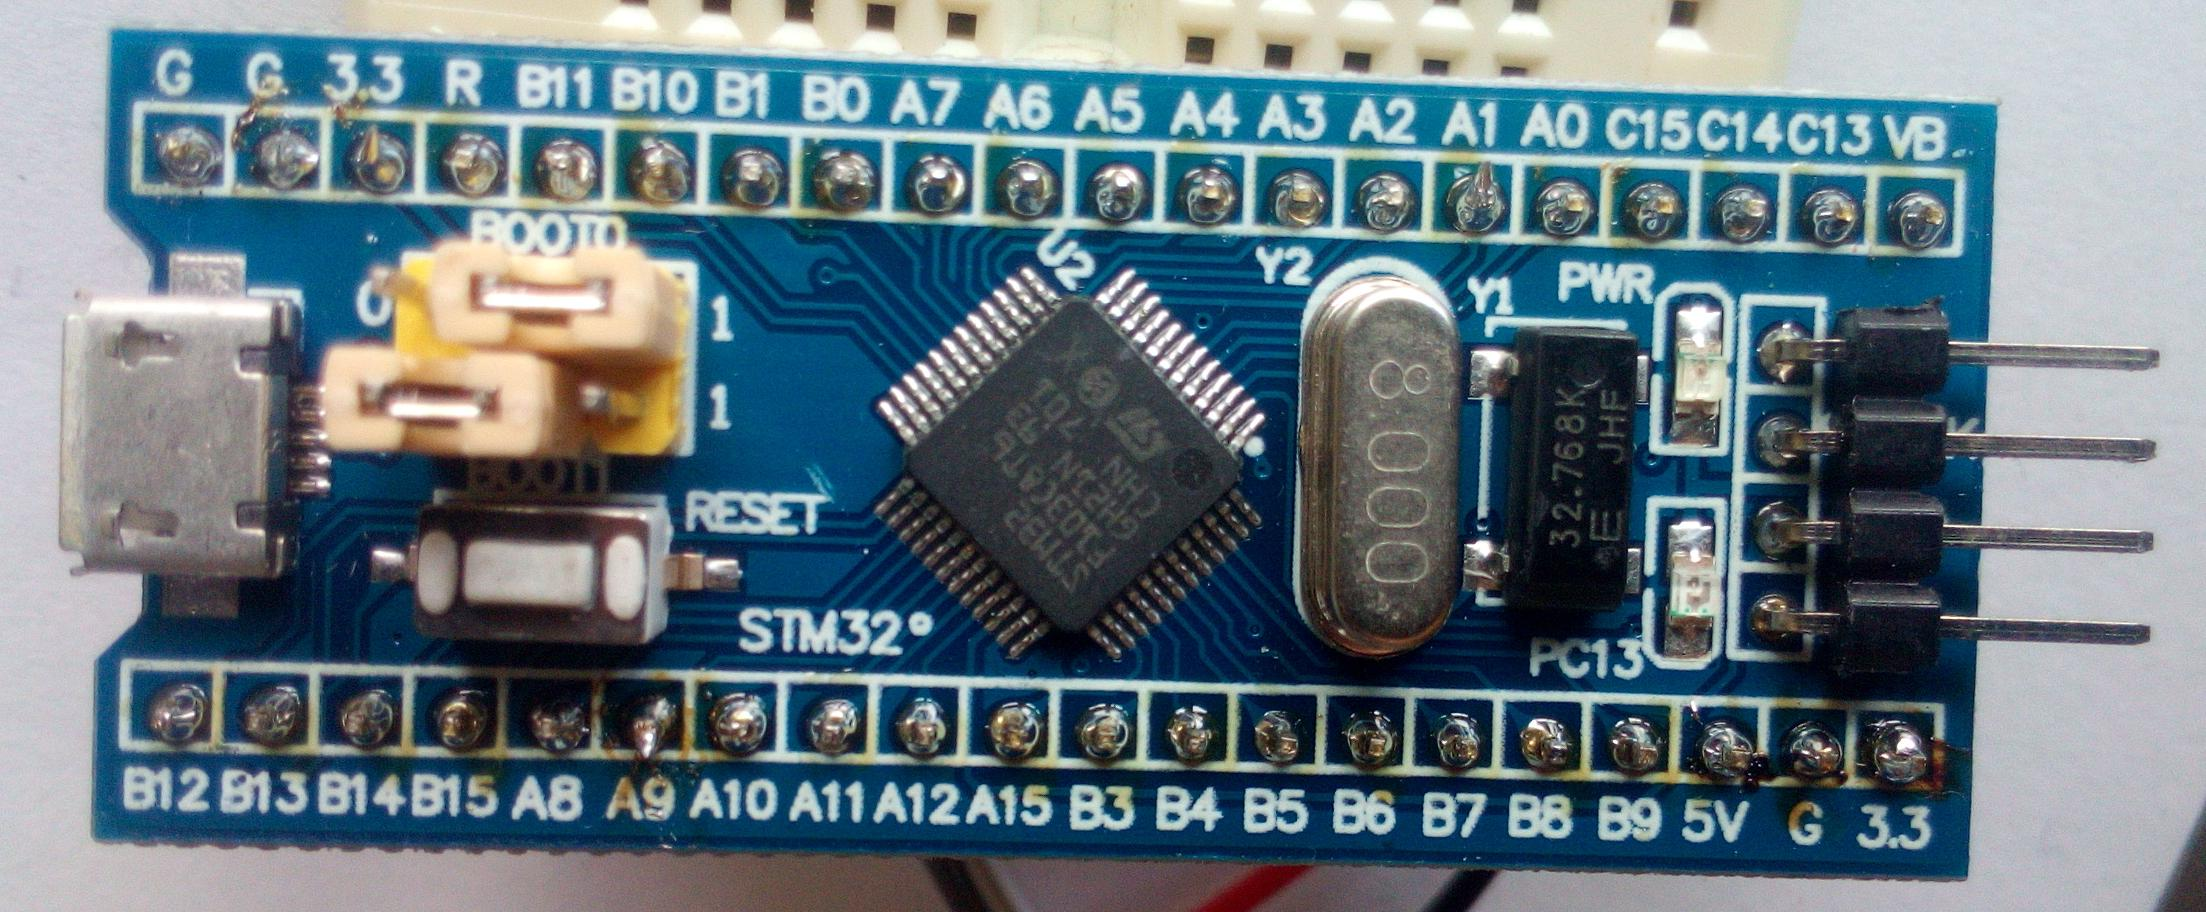
\includegraphics[height=3.3cm]{warsztat_elektroniczny/blue-pill} \end{flushright}
}


\subsection{Programator do STM32 – Konwerter USB-UART}

Do programowania użyjemy portu szerowego naszego mikrokontrolera, w celu połączenia się z nim potrzebna będzie przejściówka USB-UART. Zasadniczo dowlna tego typu przejściówka (mająca napięcia logiczne na poziomie 3.3V, czyli \textbf{nie} przejściówka typu RS232) będzie OK. Poniżej dwie przetestowane propozycje do wyboru.

\subsubsection{Moduł z układem PL2303HX}
\parbox[c]{0.55\textwidth}{
	\begin{itemize}
		\wada moduł ma wyprowadzone jedynie linie RxD i TxD
		\wada moduł do wygodnego używania wymaga przedłużacza USB
		\info od 3.5PLN
	\end{itemize}
}
\hspace{\stretch{1}}
\parbox[c]{0.43\textwidth}{
	\begin{flushright} 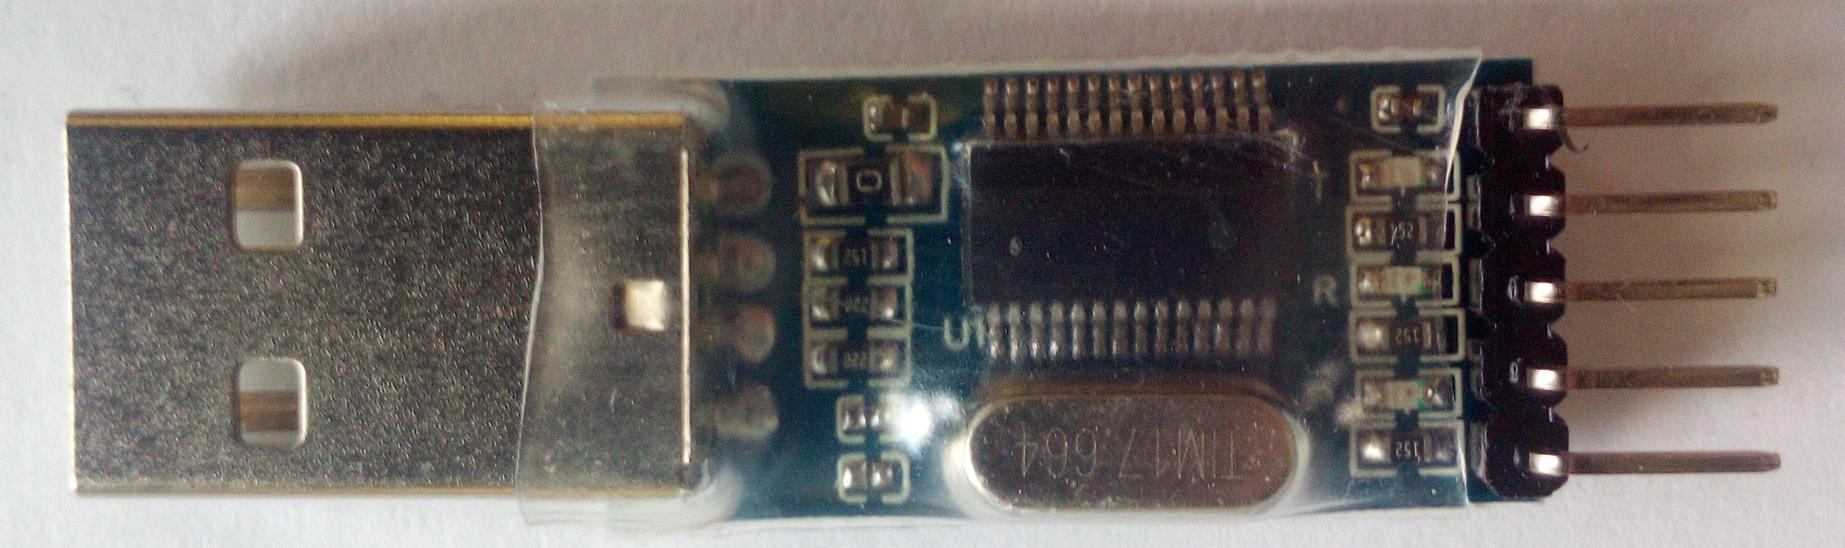
\includegraphics[height=2.3cm]{warsztat_elektroniczny/usb-uart1} \end{flushright}
}

\subsubsection{Moduł z układem FTDI FT232RL}
\parbox[c]{0.65\textwidth}{
	\begin{itemize}
		\zaleta moduł ma wyprowadzone na bocznych wszystkie linie portu szeregowego, co prawda nam nie będzie to potrzebne, ale może się przydać w innych zastosowaniach (np. programowanie układów ESP)
		\wada moduł wymaga kabla mini-usb
		\info od 10PLN
	\end{itemize}
}
\hspace{\stretch{1}}
\parbox[c]{0.33\textwidth}{
	\begin{flushright} 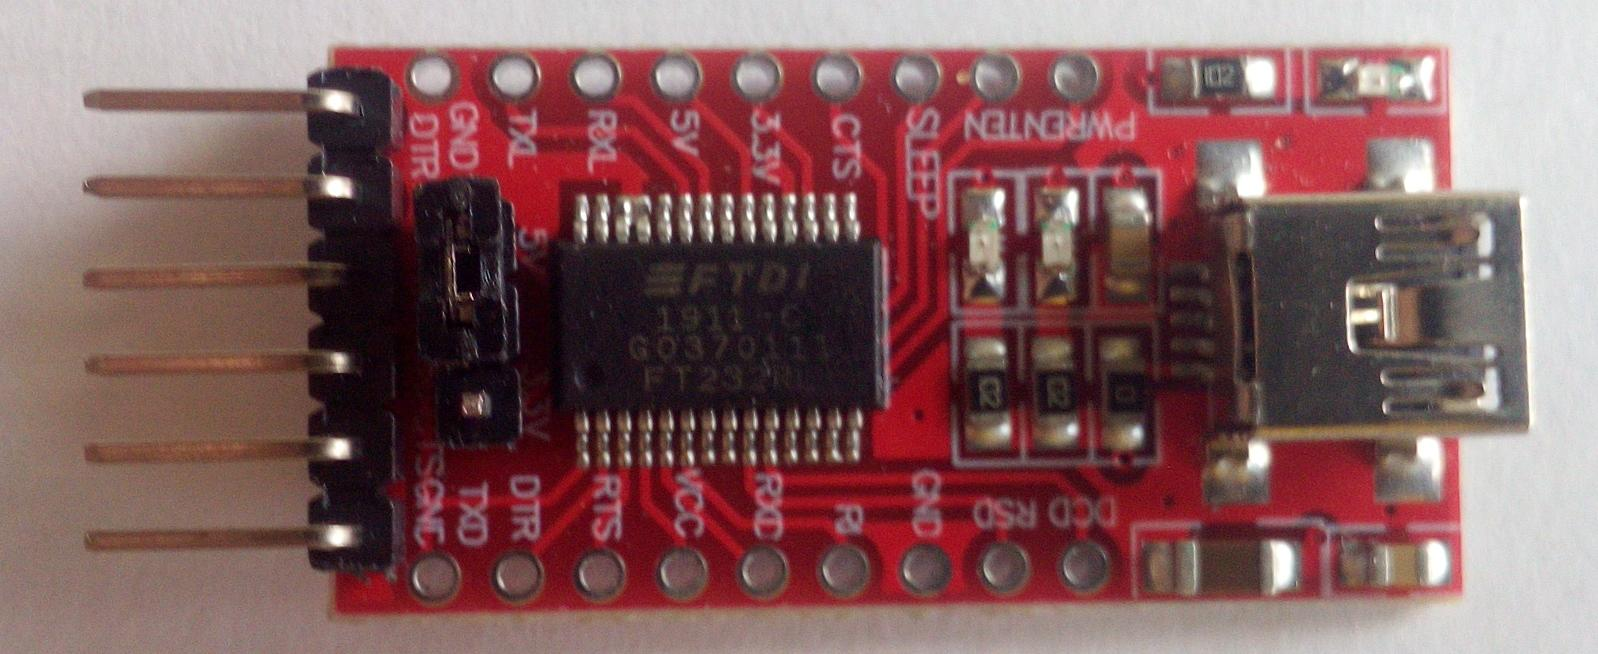
\includegraphics[height=2.3cm]{warsztat_elektroniczny/usb-uart2} \end{flushright}
}
